\documentclass[11pt,a4paper]{bxjsarticle}
\usepackage{luatexja}
\usepackage{etoolbox}
\usepackage{graphicx}
\usepackage{grffile}
\usepackage[table]{xcolor}
\usepackage{tikz}
\usepackage{textcomp}
\usepackage{amsmath}
\usepackage{amsthm}
\usepackage{amssymb}
\usepackage{mathtools}
\usepackage{bm}
\usepackage{physics}
\usepackage{cancel}
\mathtoolsset{showonlyrefs=true}
\usepackage[hang,small,bf]{caption}
\usepackage[subrefformat=parens]{subcaption}
\captionsetup{compatibility=false}
\captionsetup[subfigure]{labelformat=simple}
\renewcommand{\thesubfigure}{(\alph{subfigure})}
\usepackage{listings,color}
\definecolor{key}{rgb}{0.37, 0.08, 0.25}
\definecolor{cmt}{rgb}{0.12,0.38,0.18}
\definecolor{str}{rgb}{0.06, 0.10, 0.98}
\lstset{
    basicstyle=\ttfamily,    % 基本のスタイル
    keywordstyle=\color{key},    % キーワードのスタイル
    commentstyle=\color{cmt},    % コメントのスタイル
    stringstyle=\color{str},    % 文字列のスタイル
    identifierstyle=\color{black},    % 変数のスタイル
    rulecolor=\color{black},
    frame=single,    % フレーム
    breaklines=true,    % 自動改行
    breakatwhitespace=false,    % 自動改行の区切り
    breakindent=12pt,    % 自動改行時のインデント
    captionpos=t,    % キャプションの位置(t,b,tb)
    % escapeinside=``,    % LaTeXのエスケープキー
    numbers=none,    %行番号(none, left, right)
    firstnumber=1,    % 最初の行番号
    numbersep=5pt,    % 行番号との距離
    numberstyle=\scriptsize,    % 行番号のスタイル
    showspaces=true    % 空白をPDFに出力
    tabsize=4,    % タブのサイズ
    columns = fixed,    % 列固定
    basewidth=0.5em,    % 列の幅
    lineskip=-0.25em,    % 行間
    xleftmargin=0.1cm,    % 左余白
    xrightmargin=0.1cm,    % 右余白
}
\renewcommand{\lstlistingname}{ソースコード}
\usepackage{comment}
\usepackage{float}
\usepackage{hyperref}
\usepackage{bookmark}
\usepackage{xurl}
\hypersetup{unicode,bookmarksnumbered=true,final}



\title{\LaTeX 入門 with VSCode(仮)}
\author{2K}

\begin{document}
\maketitle

\section{はじめに}
これはVSCodeで最高の\LaTeX の環境を整えるための備忘録です。私が記憶喪失になった場合に備え、かなり丁寧に説明してあります。LaTeX、VSCodeについて知らなくても、ここに書いてある手順に従えば分かるはずです。以下注意点です。

まず、この資料は完璧でないので他の資料と見比べながら進めてもらった方が安全です。\LaTeX に関することならとりあえず\url{https://texwiki.texjp.org/}を見ておけば大丈夫でしょう。説明が雑な所も多いので分からなかったらネットで調べてください。

また、あらかじめファイル管理システム(Windowsの場合はエクスプローラー)の設定をファイル名拡張子を表示するように変更しておくと良いです。もし「ファイル」、「フォルダ」、「ディレクトリ」、「拡張子」という単語になじみがない場合は調べて理解しておきましょう。

なお、OSはWindows10を想定しています。他のバージョンのWindowsだと表示が少し違うようですが、やることは余り変わりません。友人によるとWindows11でも問題なくできたそうです。macOS、Linuxなどの場合は大きく異なる点が出てくるので十分注意してください。

最後に、これはあくまで私のための備忘録なので、これを参考にして何か問題が起こっても全て自己責任でお願いします。

\section{\TeX Live}
\subsection{\TeX Liveのインストール}
まずは\TeX Liveをパソコンにインストールします。\TeX Liveとは、簡単に言うと\LaTeX を動かすためのプログラムとかを全部まとめたものです。詳しくは \url{https://texwiki.texjp.org/?TeX%20Live} を参照してください。

Windowsの場合は\url{https://texwiki.texjp.org/?TeX%20Live%2FWindows}からインストーラをダウンロードできます。基本的にはネットワークインストーラを用いる方法で良いと思います。他のOSの場合は対応するページを見てください。

この\TeX Live、容量が3.4GB程と非常に重たいです。パソコンの空き容量は10GB以上あった方が安心です。また、インストールに1、2時間かかるので、通信環境の良い場所で時間がある時にやりましょう。

\subsection{環境変数の確認}
インストールが終わったら環境変数の確認をします。これは万全を期すための確認なので、よく分からない場合は\ref{textest}節に飛んでもらっても構いません。

Windowsの場合、タスクバーの検索ボックスに「システム環境変数」と入力してください。すると図\ref{fig:path1}のような画面が表示されるので、「システム環境変数の編集」を開いてください。「環境変数の編集」というものもありますが、これではないので気を付けてください。図\ref{fig:path2}のようなウィンドウが開いたら右下の「環境変数」をクリックします。さらに図\ref{fig:path3}のようなウィンドウが開くので、「システム環境変数」の枠内の「Path」をダブルクリックしてください。そこに

% このソースコードの部分はインデントを全て左端にしてください
\begin{quote}
\begin{verbatim*}
%SystemRoot%\system32
\end{verbatim*}
\end{quote}
と
\begin{quote}
\begin{verbatim*}
%SystemRoot%
\end{verbatim*}
\end{quote}
の2つが含まれていればOKです。なければ「新規」を押して追加してください。
\begin{figure}[H]
    \centering
    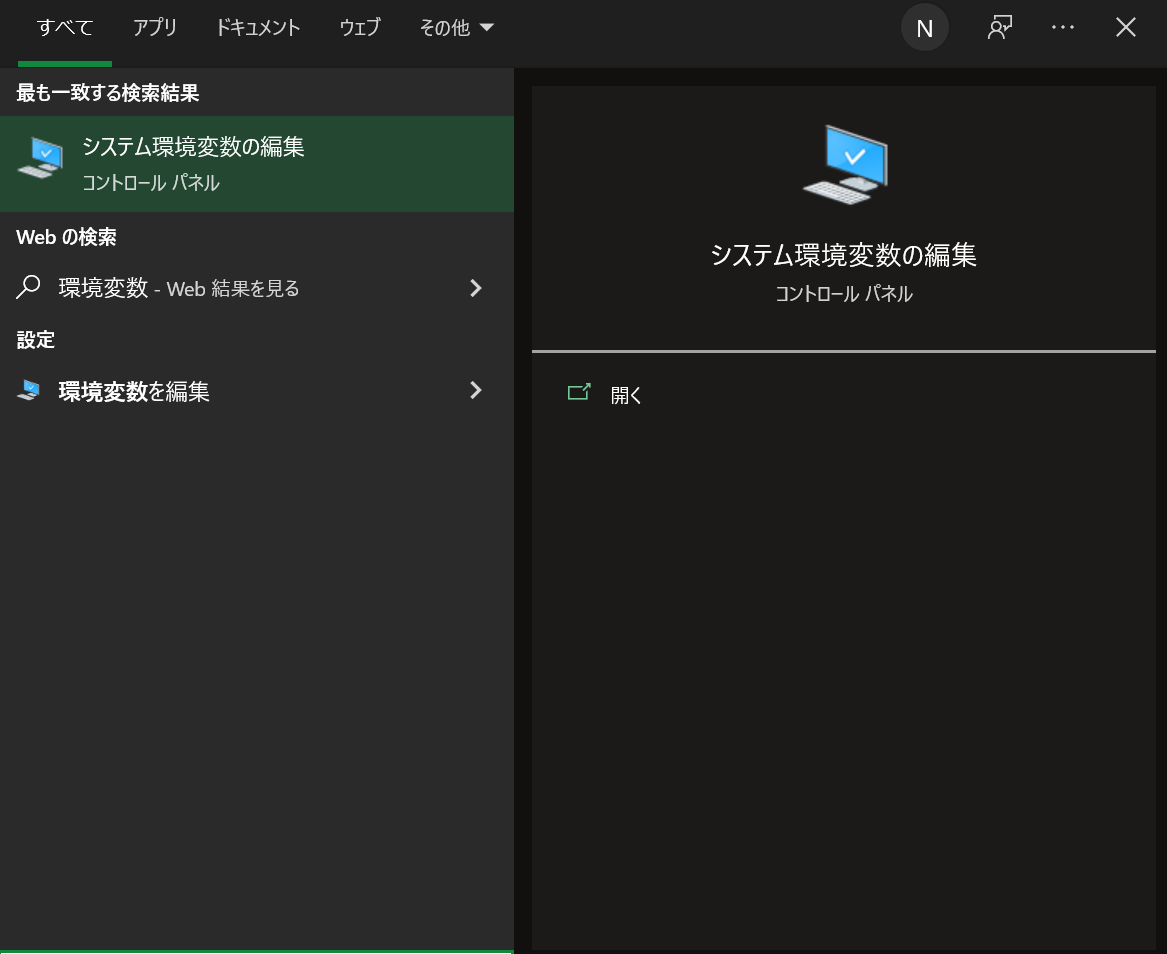
\includegraphics[height=70mm]{img/path1.png}
    \caption{}
    \label{fig:path1}
\end{figure}
\begin{figure}[H]
    \centering
    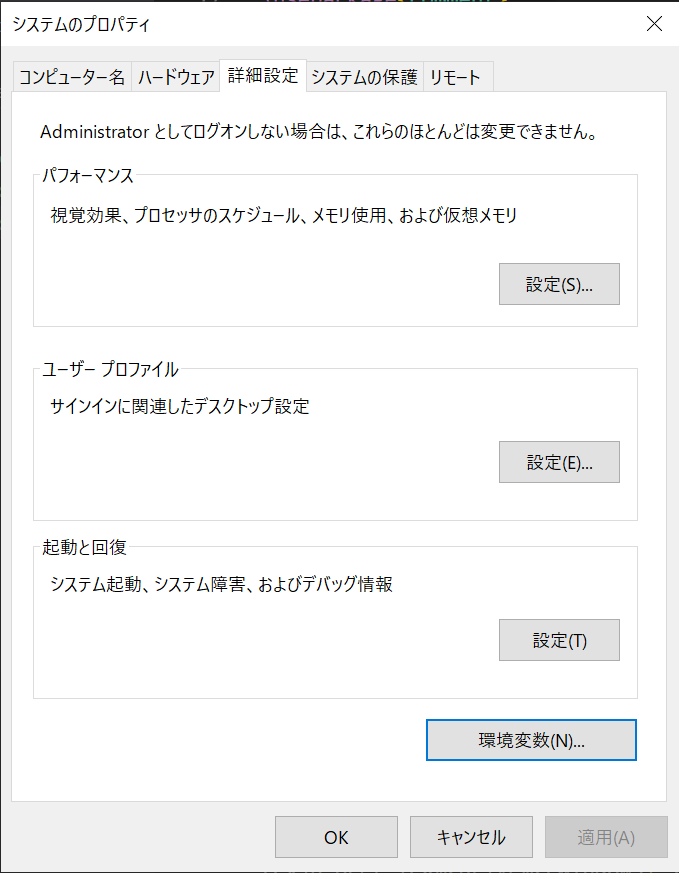
\includegraphics[height=90mm]{img/path2.png}
    \caption{}
    \label{fig:path2}
\end{figure}
\begin{figure}[H]
    \centering
    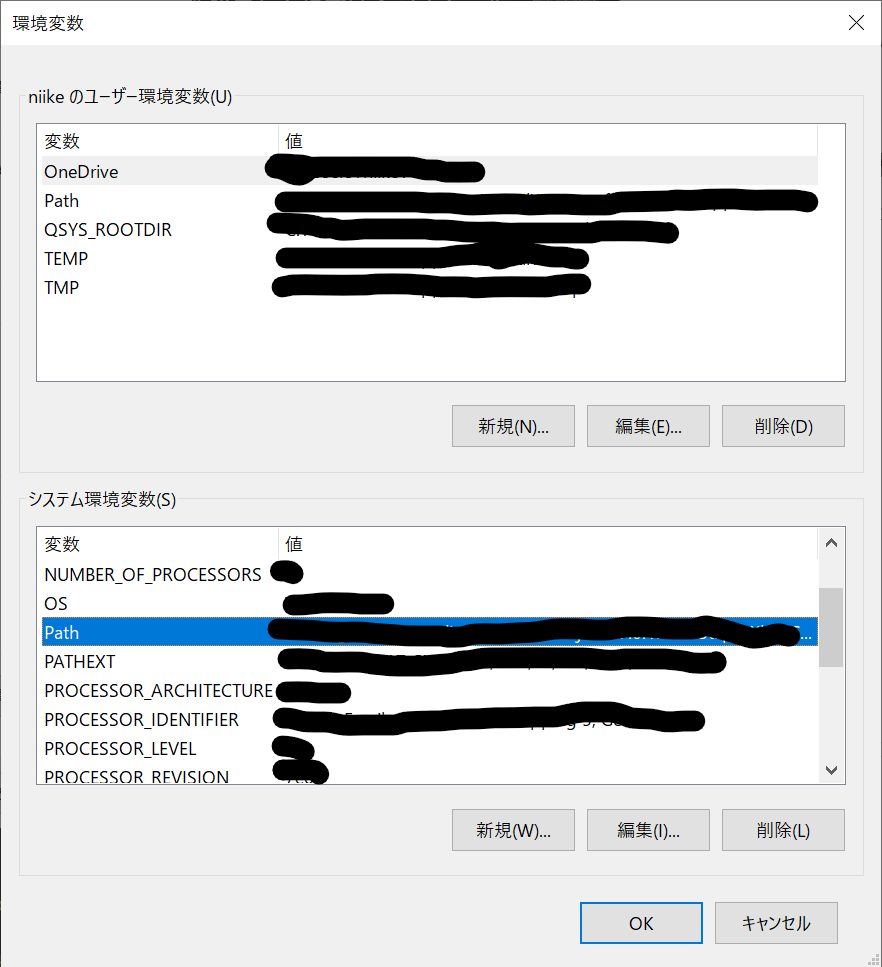
\includegraphics[height=80mm]{img/path3.png}
    \caption{}
    \label{fig:path3}
\end{figure}

\subsection{\TeX Liveのテスト}\label{textest}
次に、\LaTeX を実際に書いて\TeX Liveが正常にインストールされていることを確認します。ここではTeXworksというエディタを使います。タスクバーの検索ボックスに「texworks editor」と入力するか、スタートメニューの「TeX Live 2021」→「TeXworks editor」から起動してください。エディタが表示されたら、次のコード\ref{code:TexLiveのテストコード}を貼り付けてください。

\begin{lstlisting}[language={[LaTeX]TeX}, caption=TeXLiveのテストコード, label=code:TexLiveのテストコード]
\documentclass{article}
\begin{document}
\begin{quote}
    \begin{verbatim*}
        Hello \LaTeX !\\
        こんにちは \LaTeX !
    \end{verbatim*}
\end{quote}
\end{document}
\end{lstlisting}

左上の緑の三角のボタンを押すとファイルの保存場所を聞かれるので、適当な場所に保存してください。 ビルドが始まり、図\ref{fig:texworks1}のように表示されたら成功です。上手く行かない場合はまず入力内容が正しいか確かめ、それでもダメなら\url{https://texwiki.texjp.org/?Microsoft%20Windows}を見て指示に従ってください。

\begin{figure}[H]
    \centering
    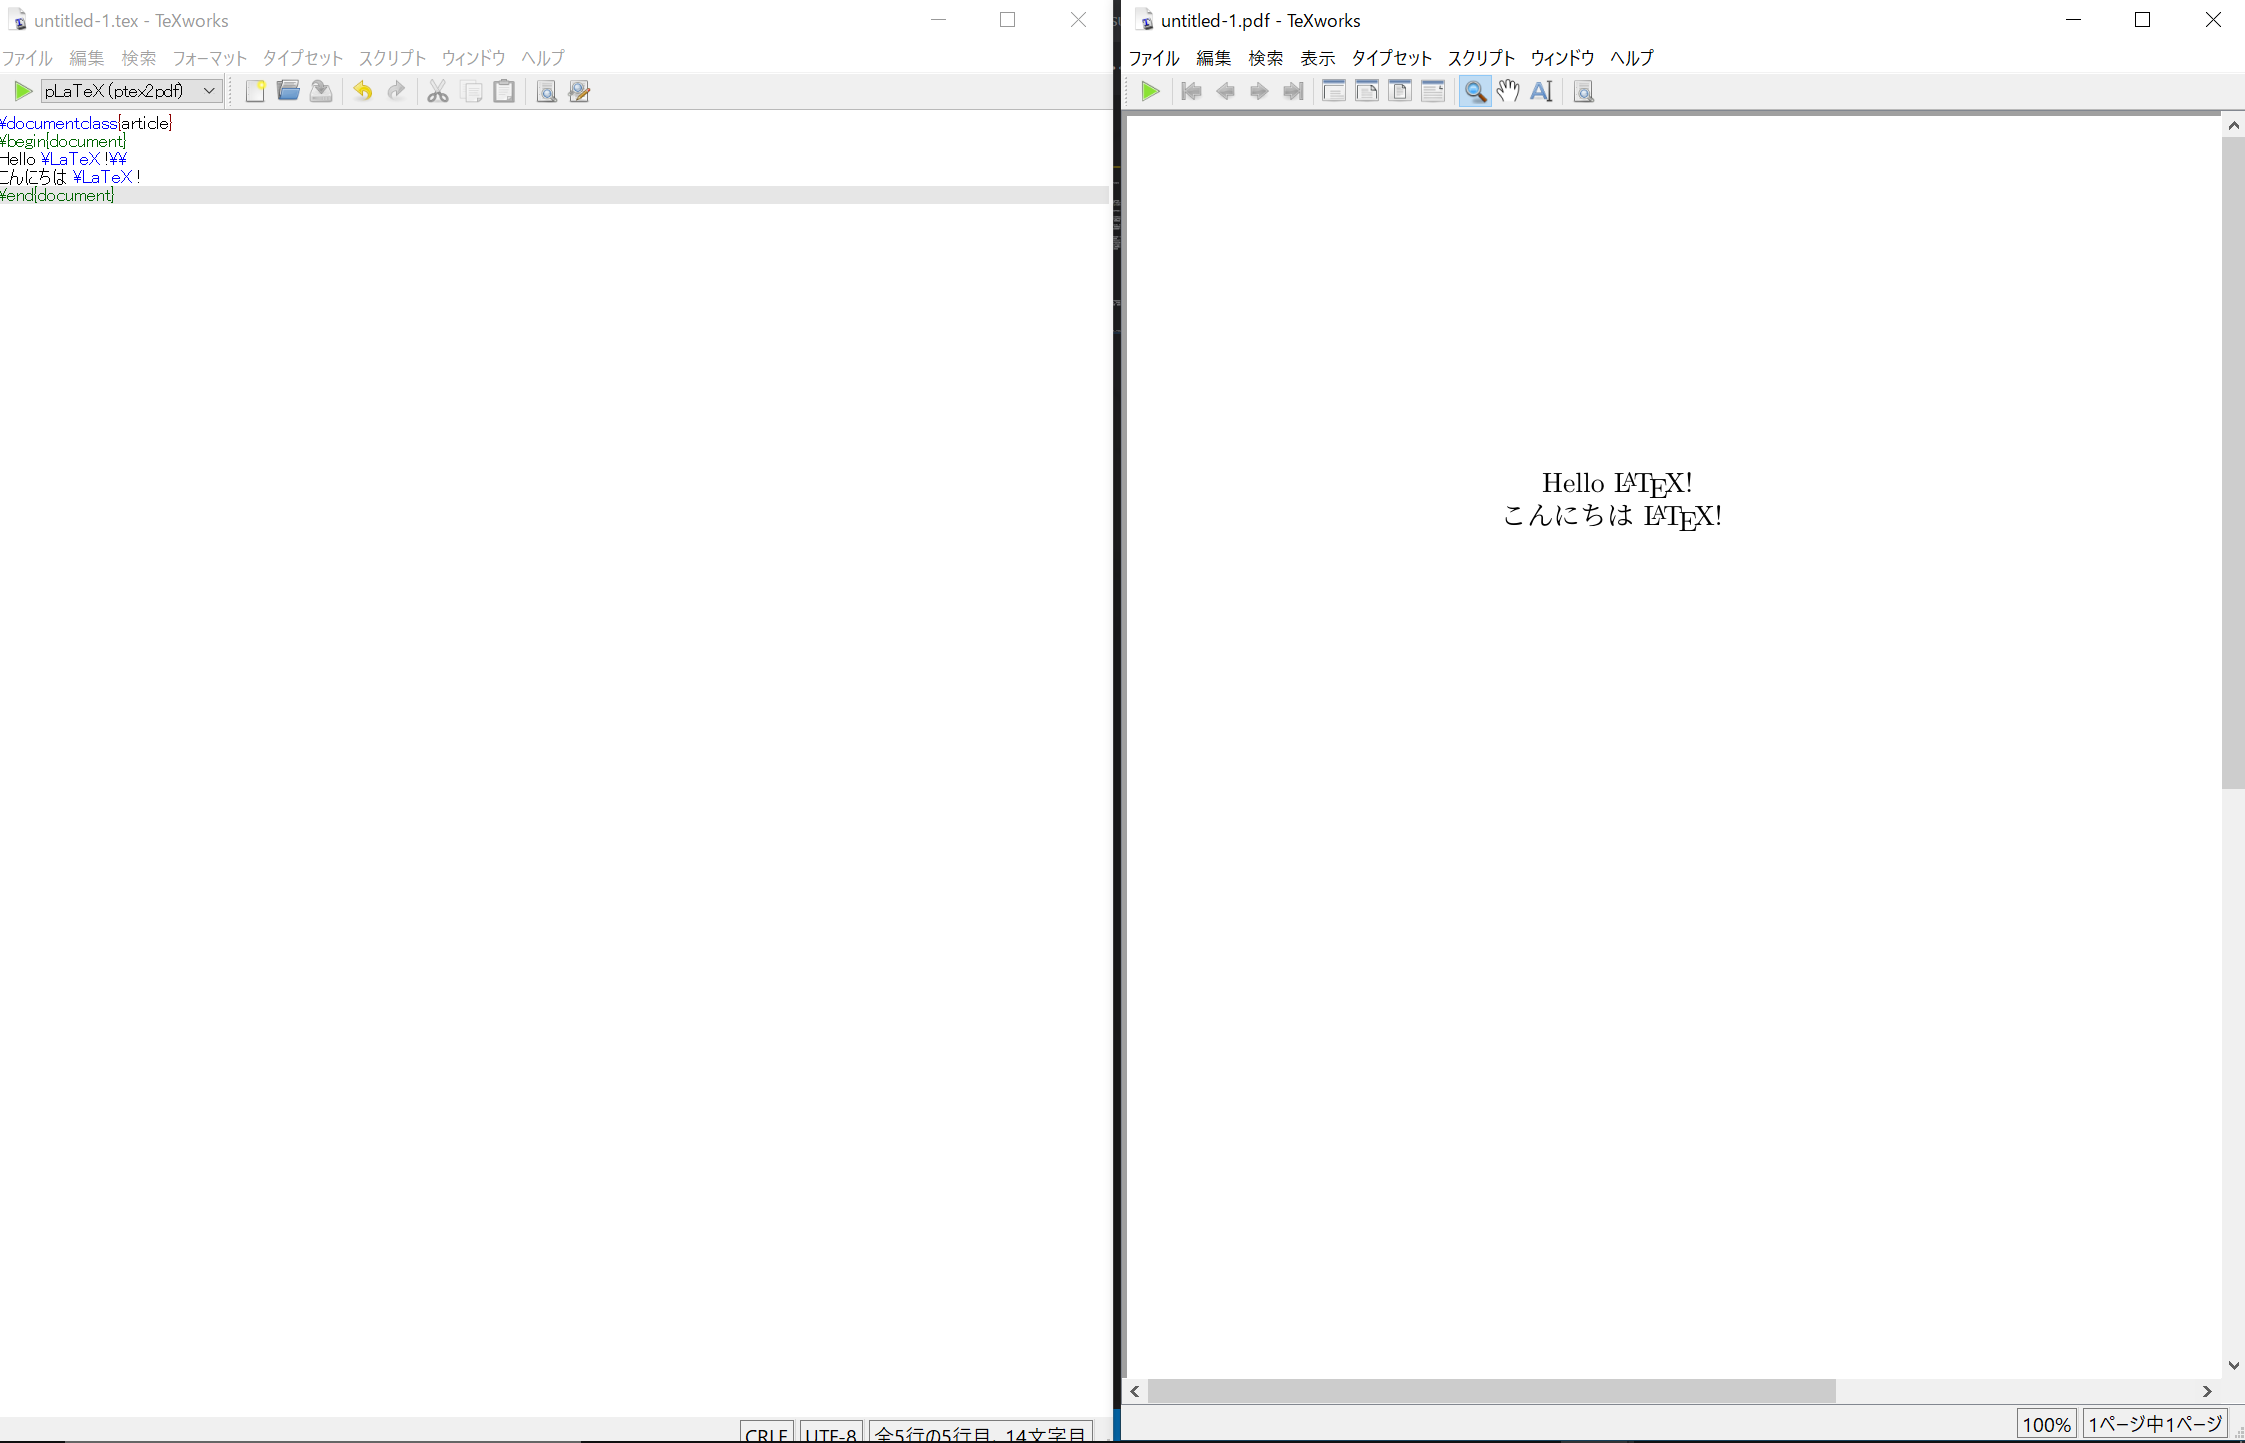
\includegraphics[height=90mm]{img/texworks.png}
    \caption{}
    \label{fig:texworks1}
\end{figure}
\LaTeX には様々なビルドの方式があります。先程の緑の実行ボタンの右に書いてあるのが現在使っている方式の名前です。クリックすると図\ref{fig:texworks2}のようになってどの方式を使うかを選択することができます。今回はLua\LaTeX という方式を使うので、「LuaLaTeX」を選択して再度実行ボタンを押し、正しくビルドされることを確認してください。問題がなければアプリを終了してもらって構いません。

\begin{figure}[H]
    \centering
    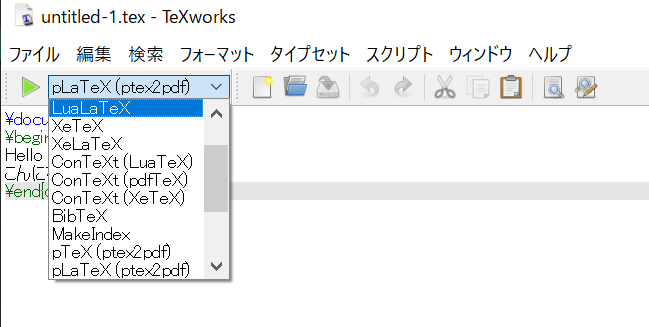
\includegraphics[height=50mm]{img/texworks2.png}
    \caption{}
    \label{fig:texworks2}
\end{figure}
これで\LaTeX 自体の設定は終わりです。この先に書いてあることをしなくても、\TeX Liveを使えばレポートを書くことはできます。ここからは、VSCodeというエディタを使って\LaTeX をよりスマートに編集する方法について説明します。

\section{VSCode}\label{sec:VSCode}
\subsection{VSCodeのインストール}\label{sec:vsinstall}
\ref{sec:VSCode}節ではVSCodeのインストール方法と基本設定について説明します。VSCodeを既に使っている場合は\ref{sec:vslatex}節に飛んでもらっても構いません。

VSCode(Visual Studio Code)は、Microsoftが提供する無料のコードエディターです。\url{https://code.visualstudio.com/download}からダウンロードできます。Windowsの場合はWindowsロゴの真下にあるボタンを押してexeファイルを適当な場所にダウンロードし、開いてください。なお、その時に英語で書かれたページに遷移するので、興味がある場合は覗いてみましょう。初心者用の解説動画があったりします。

exeファイルを開いたらインストーラーが起動します。基本的には何もいじらずに進めてもらったら良いのですが、一か所だけして欲しい設定があります。「追加タスクの選択」という画面が表示されたら、特にこだわりがなければ図\ref{fig:vssetup}のようにチェックを入れてください。
\begin{figure}[H]
    \centering
    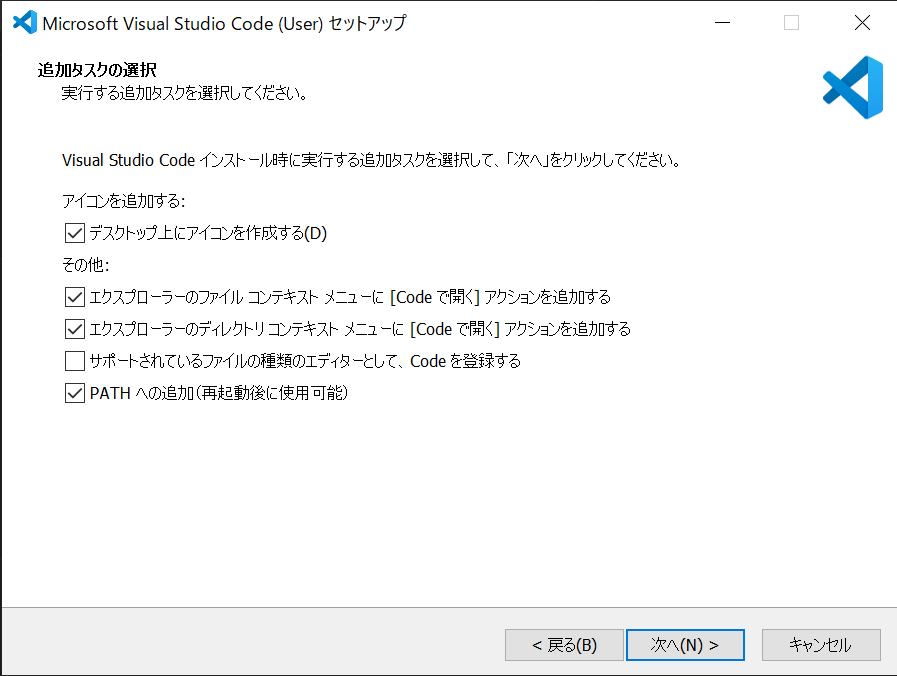
\includegraphics[height=85mm]{img/vscodesetup.png}
    \caption{}
    \label{fig:vssetup}
\end{figure}
各項目について一応説明しておきます。気になる人は読んでください。
\begin{description}
    \item[デスクトップ上にアイコンを作成する]\mbox{}\\
          そのままの意味です。
    \item[エクスプローラーのファイルコンテキストメニューに\textrm{[}Codeで開く\textrm{]}アクションを追加する]\mbox{}\\
          エクスプローラーでファイルの上で右クリックすると図\ref{fig:vscheck1}のように「Codeで開く」という選択肢が現れるようになります。これをクリックすればVSCode上でファイルを開けます。
    \item[エクスプローラーのディレクトリコンテキストメニューに\textrm{[}Codeで開く\textrm{]}アクションを追加する]\mbox{}\\
          上のことがフォルダに対してもできるようになります。これはよく使うので必ずチェックを付けましょう。
    \item[サポートされているファイルの種類のエディターとして、Codeを登録する]\mbox{}\\
          VSCodeで開けるファイルをダブルクリックすると、直接VSCodeで開くようになります。VSCodeを既定のエディタとして利用するならチェックを付けても良いですが、別に付けなくても構いません。迷うようならチェックははずして良いでしょう。
    \item[PATHへの追加(再起動後に使用可能)]\mbox{}\\
          コマンドプロンプトで \verb|code| と打つとVSCodeを起動できるようになります。また、 \verb*|code <ファイル名>| でファイルを、 \verb*|code -r <フォルダ名>| でフォルダを開けるようになります。よく分からなくてもとりあえずチェックを入れておいて大丈夫です。
\end{description}
\begin{figure}[H]
    \centering
    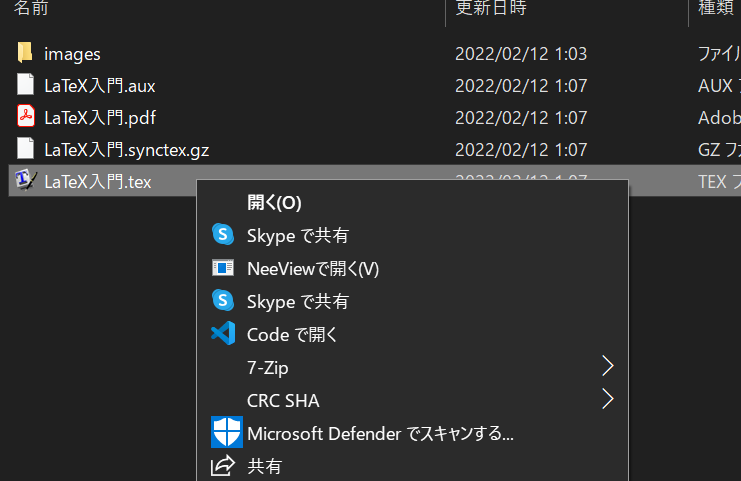
\includegraphics[height=60mm]{img/vscodecheck1.png}
    \caption{}
    \label{fig:vscheck1}
\end{figure}

チェックの入れ忘れ、間違いなどがあり後で訂正したい場合は、VSCodeをアンインストールすることなく、もう一度インストーラを開いて設定し直してください(未確認)。

\subsection{VSCodeの日本語化}
インストールが終わったら自動的にVSCodeが起動します。起動しない場合、デスクトップのアイコンをダブルクリックするか、タスクバーの検索欄に「vscode」と入力するなどして立ち上げてください。

次に、VSCodeの日本語化のための拡張機能を入れます(もちろん入れなくても構いません)。左端にあるアイコンの列の中から、田んぼの「田」の右上が切り離された感じのアイコンをクリックしてください。すると検索欄が出てくるので、「japanese」と入力して一番上に出てくる「Japanese Language Pack for Visual Studio Code」をインストールしてください(図\ref{fig:vsjp})。
\begin{figure}[H]
    \centering
    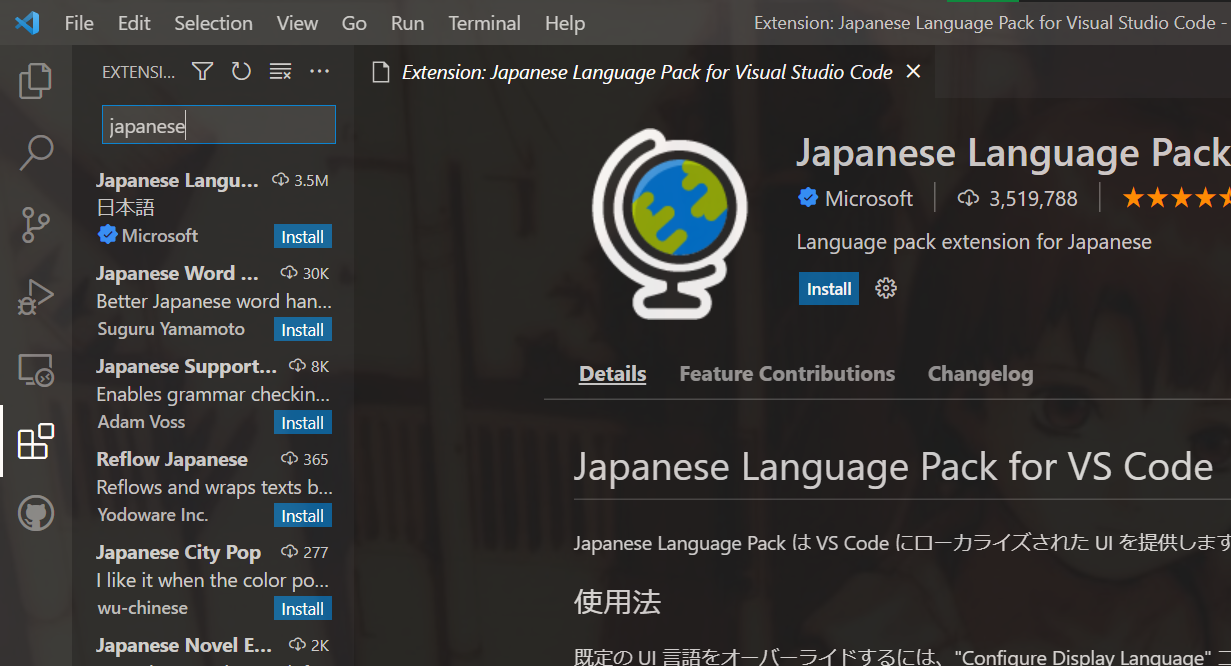
\includegraphics[height=65mm]{img/vsjp.png}
    \caption{}
    \label{fig:vsjp}
\end{figure}
すると画面の右下に英語が書かれたボタンが出てくるので、リロードして日本語化を有効にするボタンを押してください。画面に日本語が表示されればOKです。上手く行かない場合は、図\ref{fig:vsjp}の画面に戻ってそこに書いてある「使用法」に従ってください。

\section{\LaTeX \ with VSCode}\label{sec:vslatex}
\subsection{拡張機能のインストールとsettings.jsonの編集}\label{subsec:latexworkshop}
次はVSCode上で\LaTeX を動かす準備をします。まずは必要な拡張機能をインストールしましょう。拡張機能のボタンを押して「latex」と検索し、「LaTeX Workshop」をインストールしてください(図\ref{fig:latexworkshop})。

\begin{figure}[H]
    \centering
    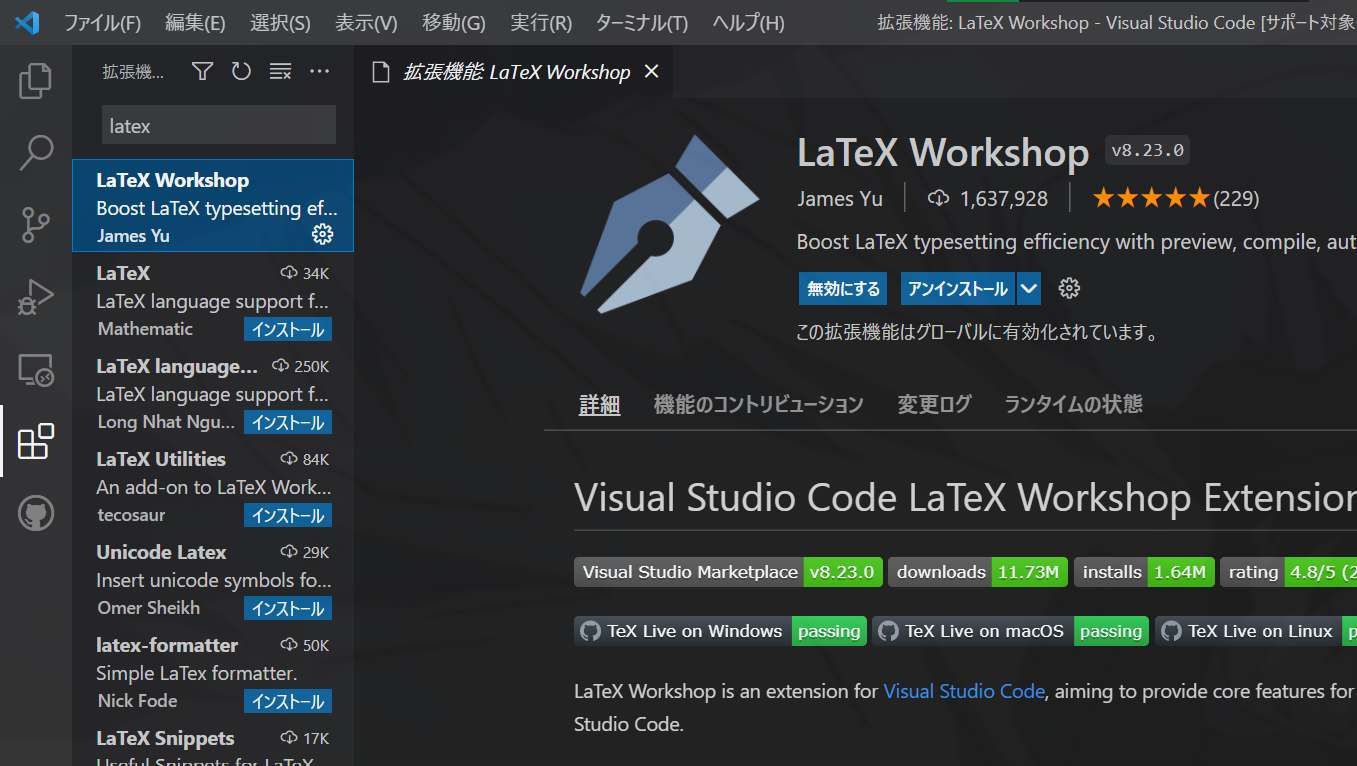
\includegraphics[height=65mm]{img/latexworkshop.png}
    \caption{}
    \label{fig:latexworkshop}
\end{figure}

次に、settings.jsonにLaTeXの設定を追加します。settings.jsonとはVSCodeのユーザー設定が記述されたファイルです。このファイルを編集することでVSCodeを自由にカスタマイズすることができます。

Ctrl+Shift+Pを押すと画面上部に検索欄(コマンドパレット)が出てくるので、そこに「設定」と入力しましょう。すると図\ref{fig:settings_json}のように設定関係の操作の候補が出てくるので、その中から「基本設定: 設定(JSON)を開く」を選択します。「既定の設定(JSON)を開く」とは別物なので注意してください。

\begin{figure}[H]
    \centering
    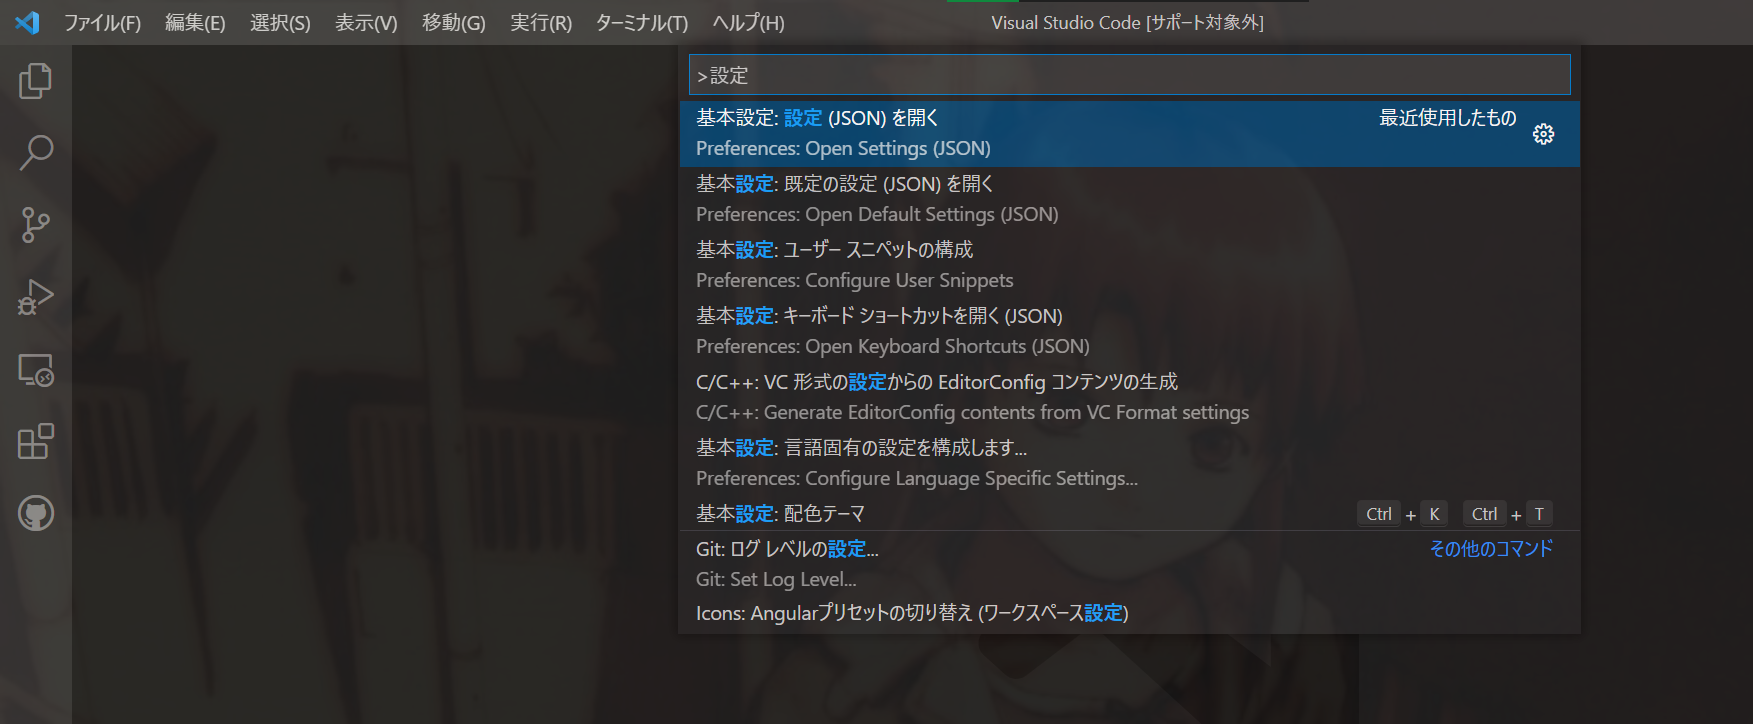
\includegraphics[height=50mm]{img/settings_json.png}
    \caption{}
    \label{fig:settings_json}
\end{figure}

すると、settings.jsonというファイルが開きます。まだ何も設定をしていない場合、空欄か中身がない中括弧だけが表示されると思います。

このファイルでは次のように設定を記述します。

\begin{quote}
    \begin{verbatim}
{
    "<設定1の名前>": <設定1の内容>,
    "<設定2の名前>": <設定2の内容>,
    ...
}
\end{verbatim}
\end{quote}

一番外側の中括弧と、各設定の間のカンマを忘れないように注意してください。詳しくはjson形式についてネットで調べてください。

settings.jsonが空欄の場合は、ソースコード\ref{code:stdjson}
を貼り付けて挙動を確認しましょう。これにはVSCodeの基本的な設定が記述されています。VSCode上でカーソルを重ねると各設定についての説明が読めます。

\lstinputlisting[caption=settings.jsonの基本的な例, label=code:stdjson]{src/stdsettings.jsonc}

次に、settings.jsonに\LaTeX を動かすための設定を追加します。

ソースコード\ref{code:stdjson}を先程貼り付けた場合は、ソースコード\ref{code:latexjson}の最初と最後の中括弧を削除して、コメントで指定されている場所に貼り付けてください。そうでない場合もjson形式に従って適宜追加してください。

settings.json上でカーソルを重ねると各設定についての説明が表示されます。詳細は\url{https://texwiki.texjp.org/?Visual%20Studio%20Code%2FLaTeX}などで調べてください。
\lstinputlisting[caption=settings.jsonの\LaTeX の設定, label=code:latexjson]{src/mysettings.jsonc}


\subsection{VSCodeで\LaTeX のテスト}
以上で基本的な設定は終わりです。早速VSCodeで\LaTeX を動かしてみましょう。
エクスプローラーで適当な場所にフォルダを作成し、それを右クリックして「Codeで開く」を選択して下さい。VSCodeが起動します。左上に開いているフォルダの名前が表示されるので、それをクリックして「新しいファイル」を選択してください(図\ref{fig:vsnewfile})。適当な名前(test.texなど)を付けてEnterキーを押すとファイルが作成されます。

\begin{figure}[H]
    \centering
    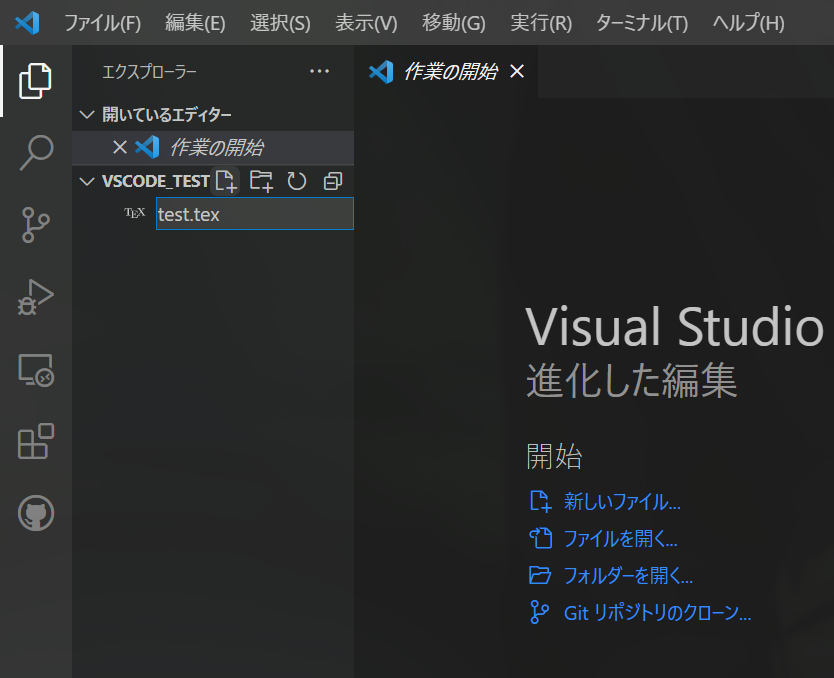
\includegraphics[height=50mm]{img/vscodetest0.png}
    \caption{}
    \label{fig:vsnewfile}
\end{figure}

作成したファイルにソースコード\ref{code:VSCodeのテストコード}を貼り付け、右上にある緑の三角のボタンを押してください。

\lstinputlisting[language={[LaTex]TeX}, caption=VSCodeのテストコード, label=code:VSCodeのテストコード]{src/vstest.tex}


上手くビルドされると左下にチェックマークが表示されます。実行ボタンの右隣のボタンを押すと、画面の右側にpdfファイルが表示されます(図\ref{fig:vscompile})。

\begin{figure}[H]
    \centering
    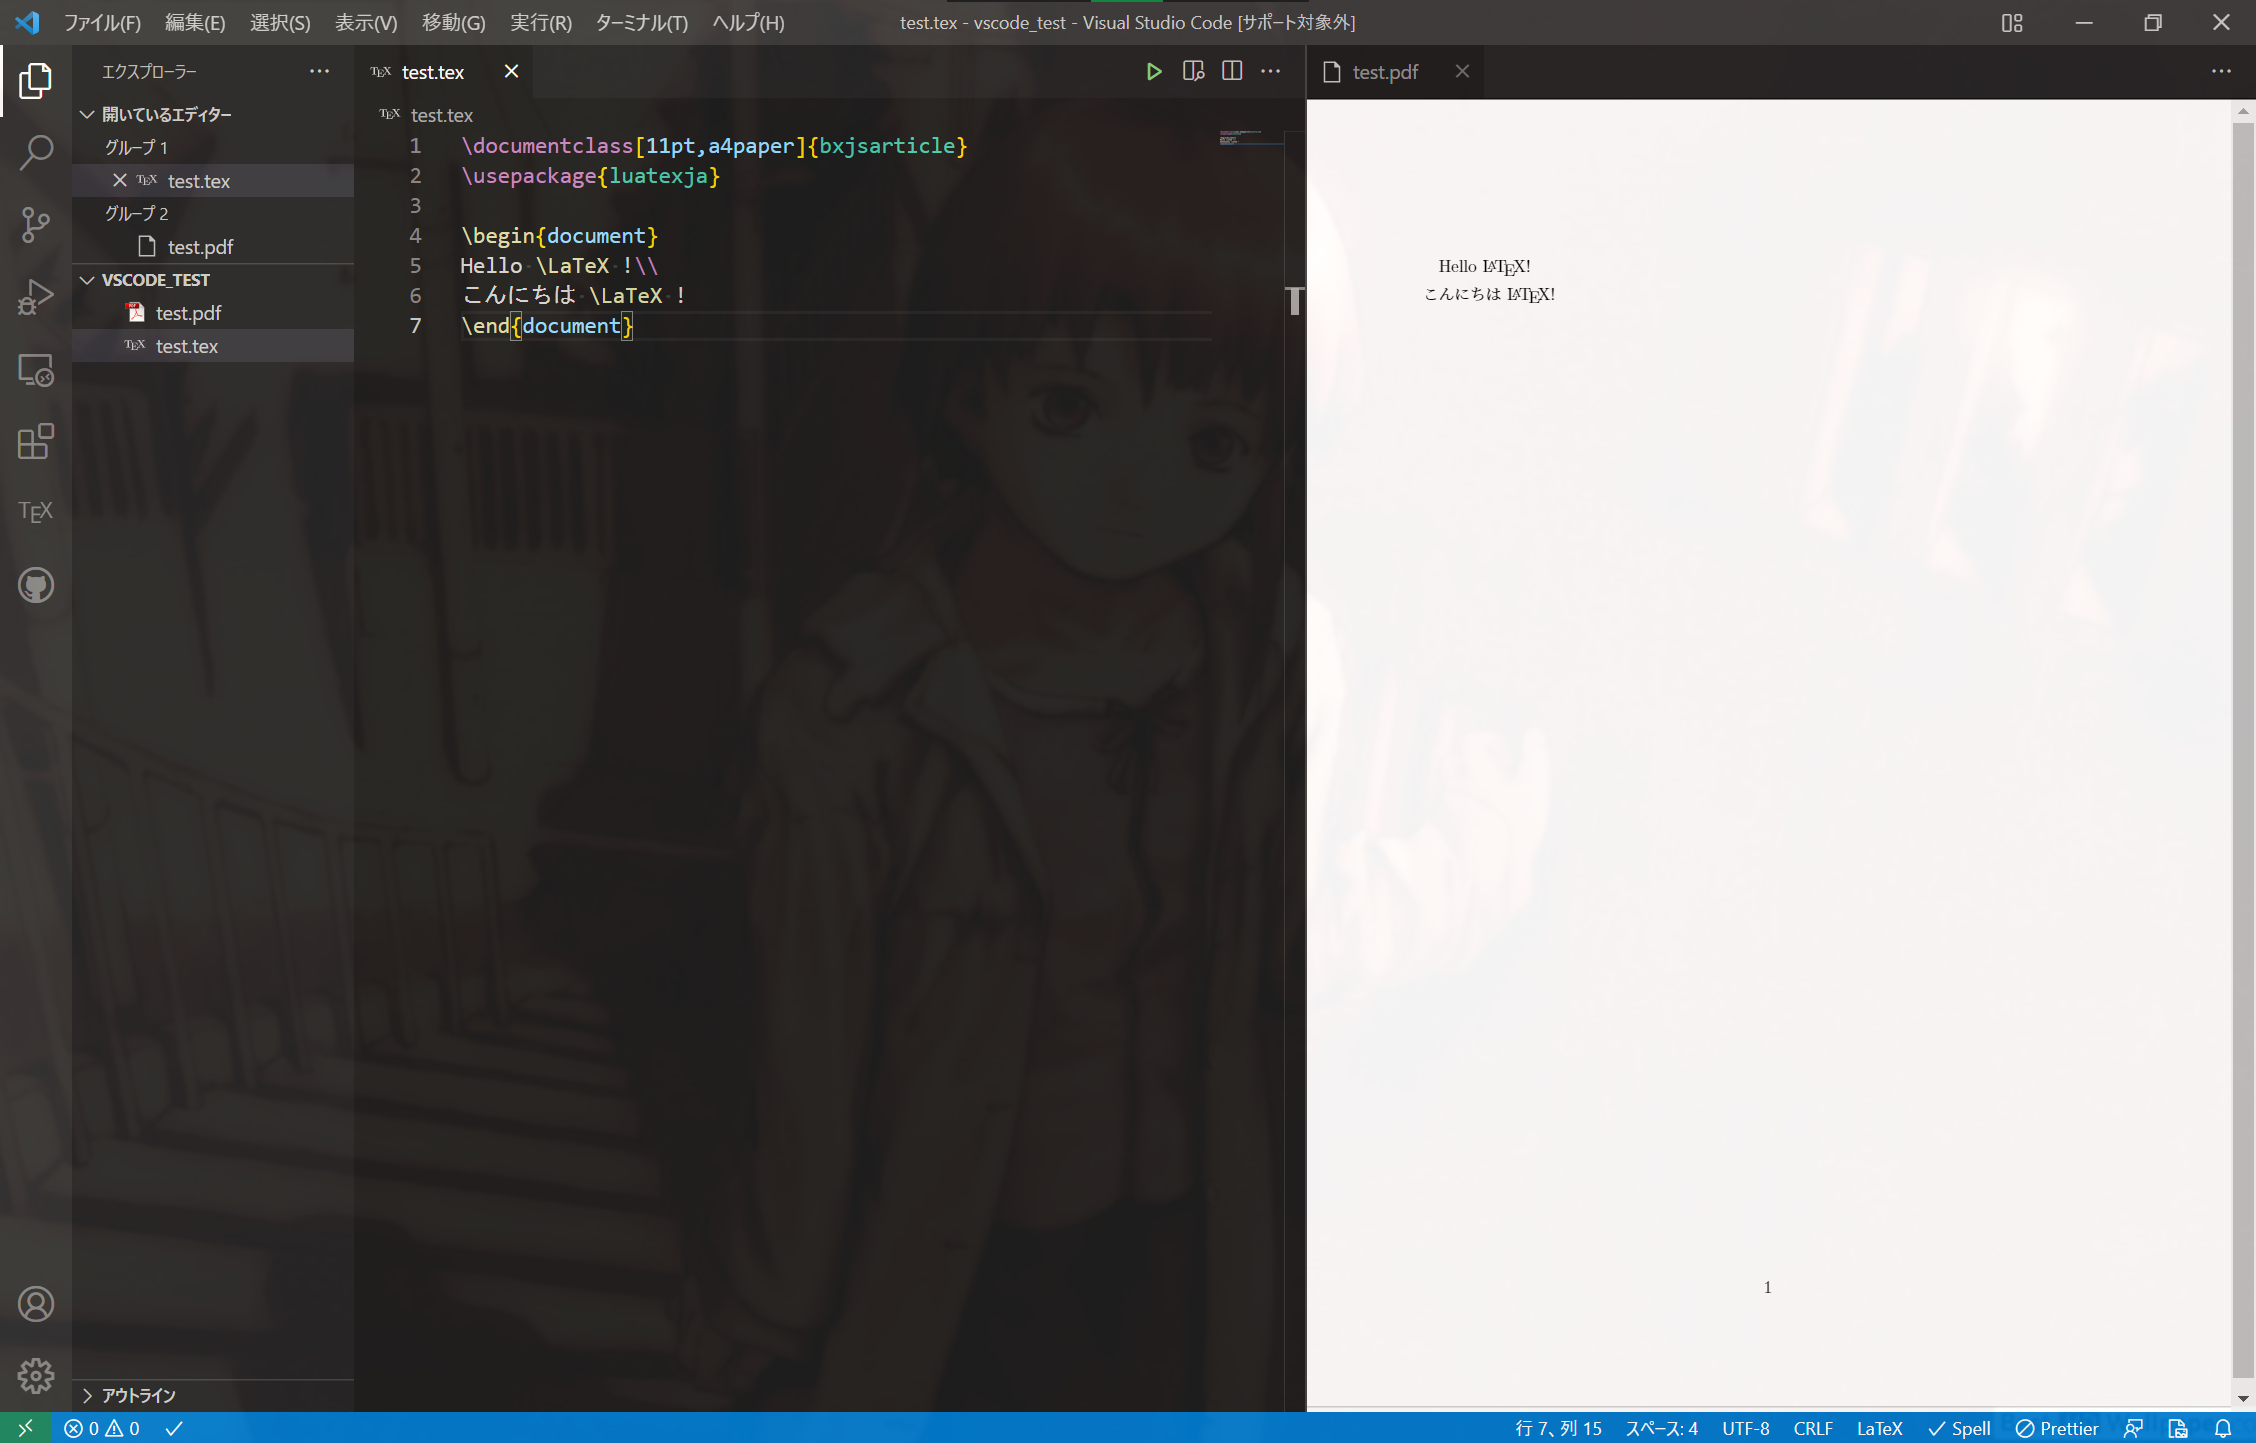
\includegraphics[height=50mm]{img/vscodetest1.png}
    \caption{VSCodeでのビルド}
    \label{fig:vscompile}
\end{figure}

pdfファイルをCtrl+左クリックすると、texファイルの対応する箇所に飛べます。逆に、texファイルでCtrl+Alt+Jを押すとpdfファイルに飛べます(Sync\TeX の機能)。

settings.jsonにソースコード\ref{code:stdjson}を貼り付けた場合、VSCodeでファイルを編集すると自動で保存が行われます。また、\ref{subsec:latexworkshop}節でインストールした拡張機能「LaTeX Workshop」の既定の設定ではファイルを保存する度にtexファイルのビルドが行われることになっています。これらの組み合わせにより、texファイルを書き換えると実行ボタンを押さなくても自動でpdfファイルが更新されることになります。自動保存、自動ビルドが嫌な場合は各自で設定を変更してください。(refなどの相互参照を使う場合、2回ビルドが必要になります。詳しくは調べてください。)

\section{\LaTeX の執筆}
\subsection{プリアンブルについて}
書けたら書く

\subsection{スニペットの活用}
書けたら書く

\subsection{Gitの活用}
書けたら書く

\section{おまけ: VSCodeの便利機能}
\subsection{コマンドパレットについて}\label{ssec:cmp}
VSCodeでCtrl+Shift+Pを押すと、画面の上部にコマンドパレットが表示されます。ここにやりたいことを入力するとたいていの事ができます。例えば「ファイル」と入力すれば図\ref{fig:vscmp}のようにファイルに関する操作の一覧が表示されます。

VSCodeを再起動したいなら「reload」と入力しましょう。図\ref{fig:reload}のような画面が開き、上下キーで操作を選択できます。「開発者: ウィンドウの再読み込み」の上でEnterキーを押すかクリックすれば、VSCodeを再起動できます(正確には再起動ではなく再読み込み?)。このように、コマンドパレットを使えば直感的な操作を行うことが可能となります。
\begin{figure}[H]
    \centering
    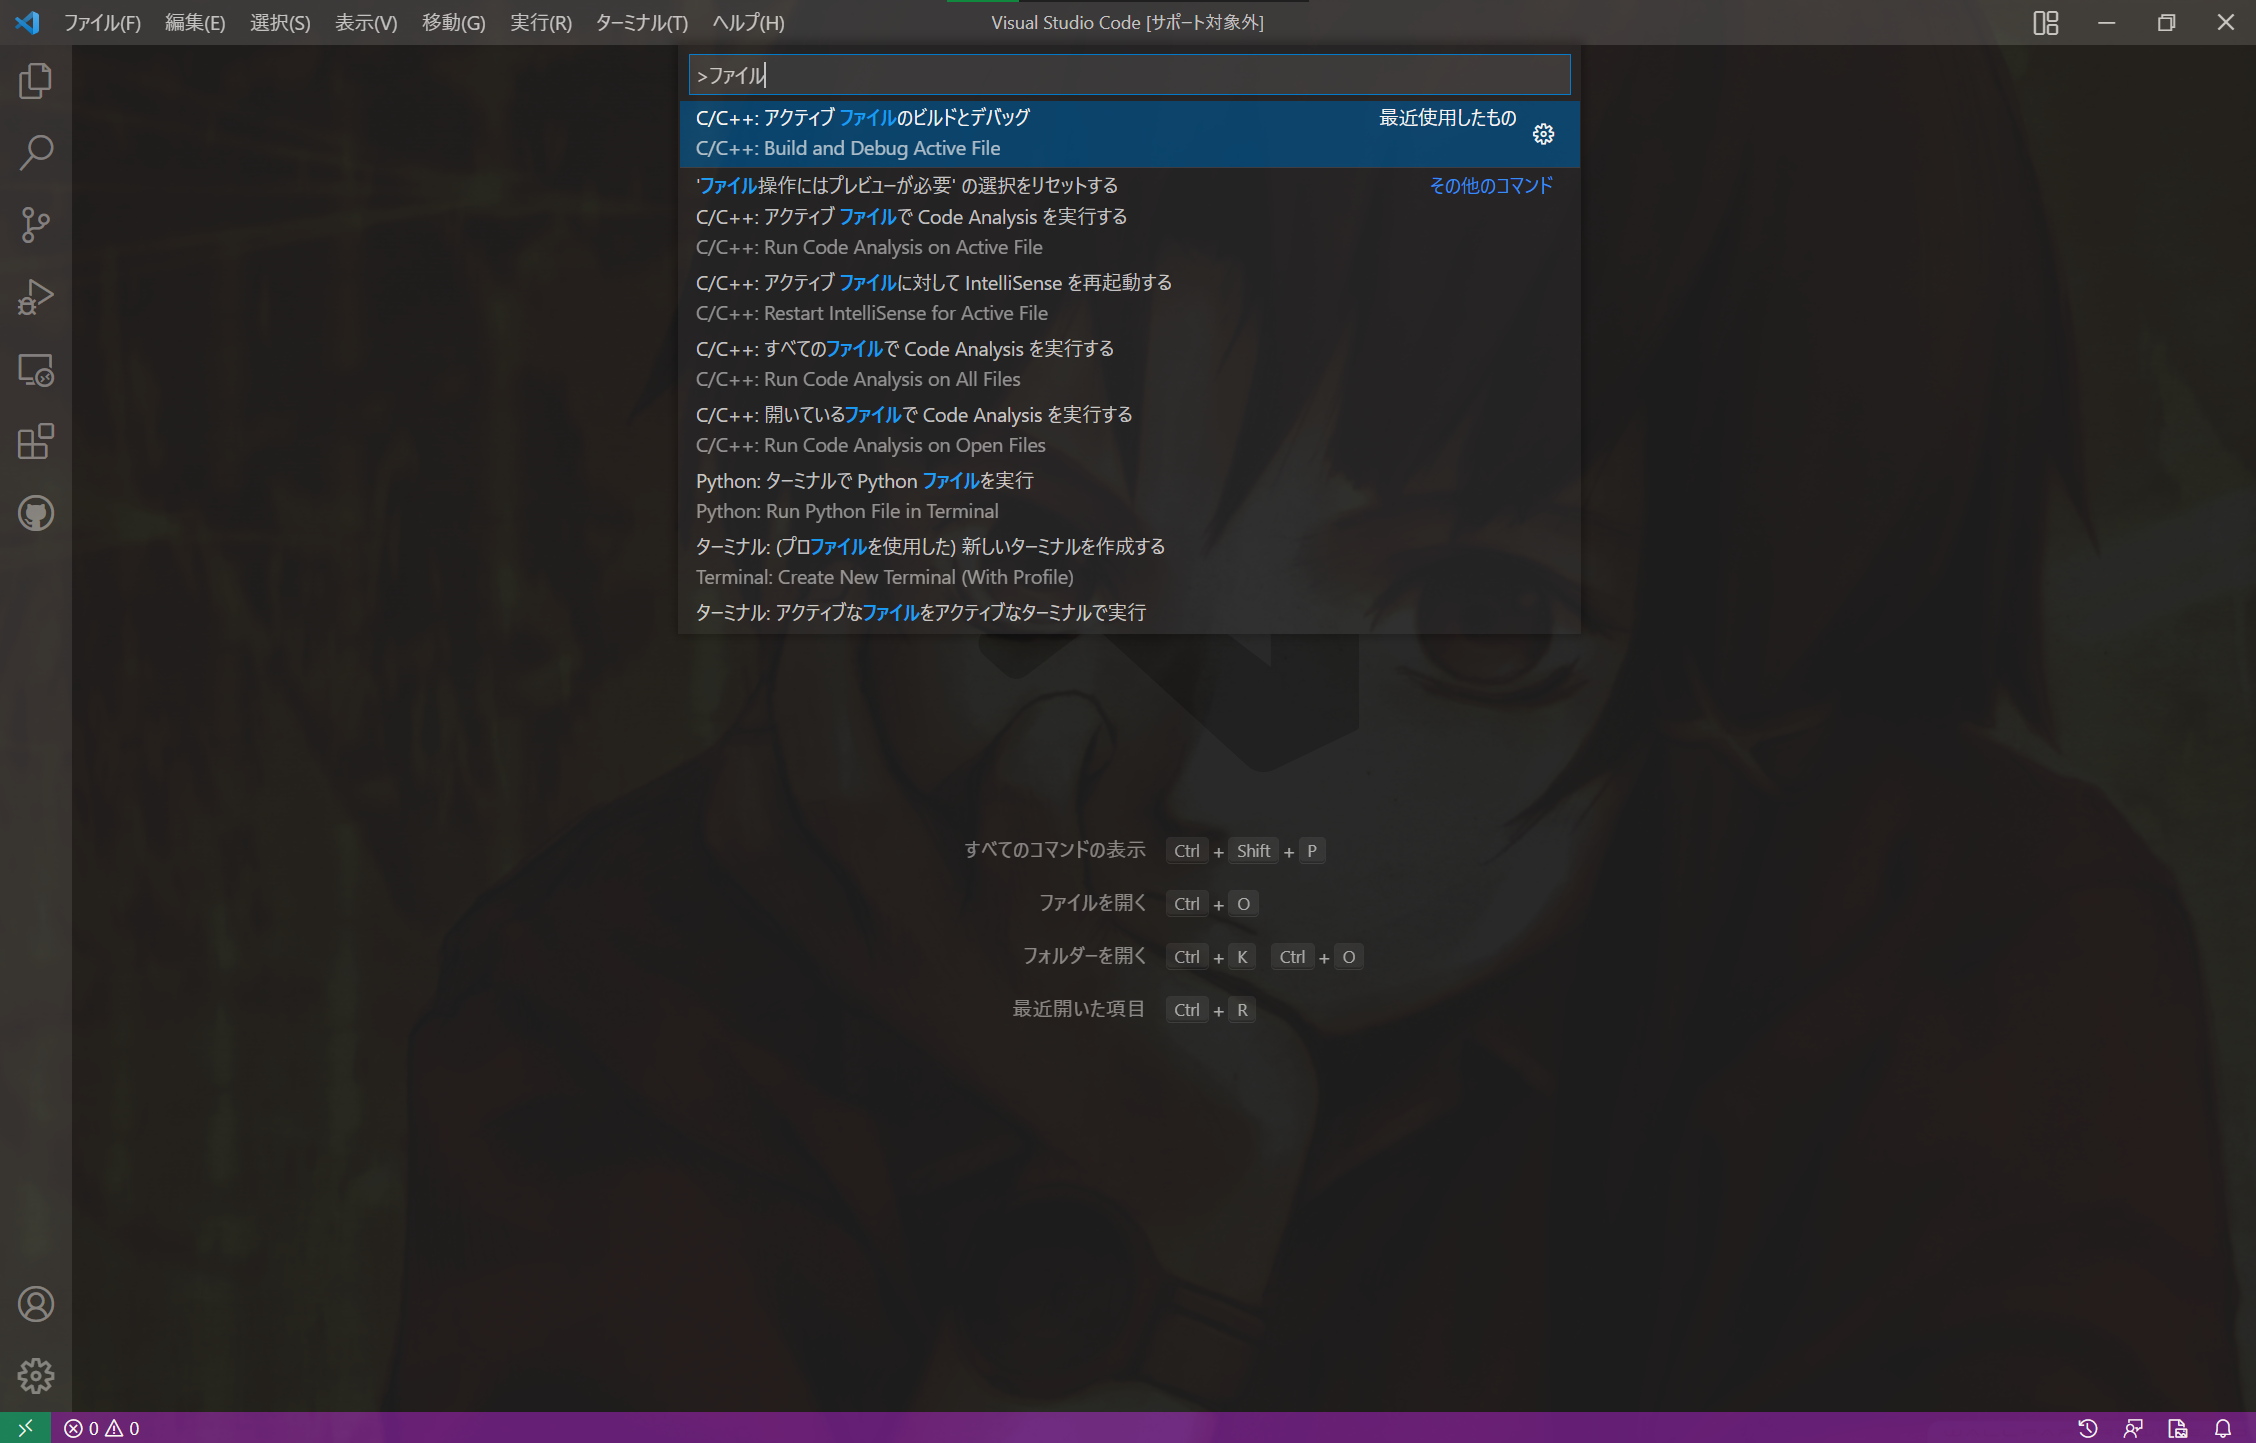
\includegraphics[height=70mm]{img/vscmp.png}
    \caption{}
    \label{fig:vscmp}
\end{figure}

\begin{figure}[H]
    \centering
    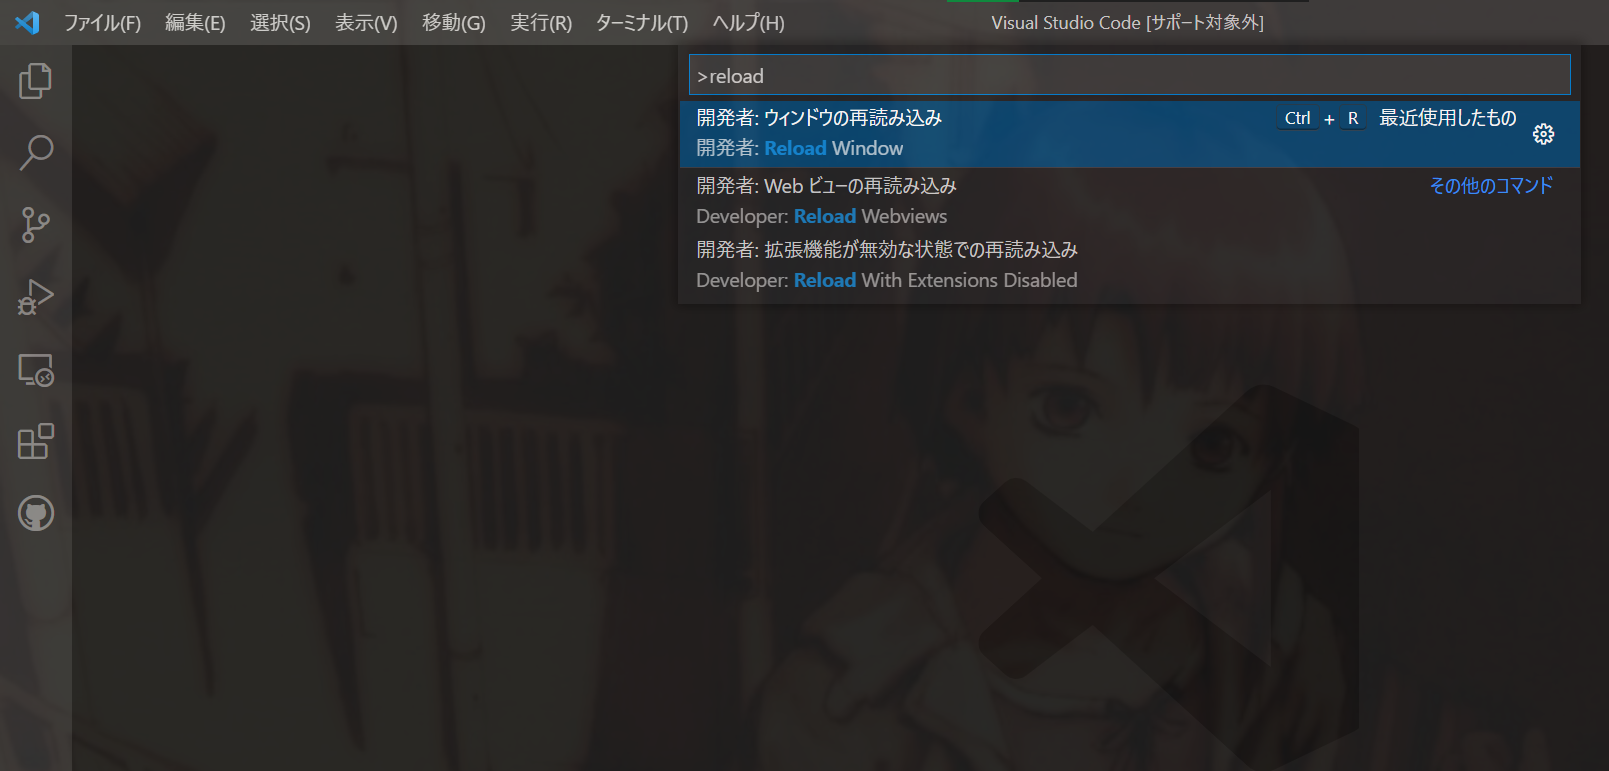
\includegraphics[height=50mm]{img/reload.png}
    \caption{}
    \label{fig:reload}
\end{figure}

\subsection{拡張機能について}
背景画像を設定したければ、「background\footnote{\url{https://marketplace.visualstudio.com/items?itemName=shalldie.background}}」か「background-cover\footnote{\url{https://marketplace.visualstudio.com/items?itemName=manasxx.background-cover}}」が良いです。私は「background-cover」を入れています。ただ、どちらを入れてもたまにエラーが出るようになります。特に害はなさそうですが、結構邪魔です。「Fix VSCode Checksums\footnote{\url{https://marketplace.visualstudio.com/items?itemName=lehni.vscode-fix-checksums}}」を入れるとそのエラーを無視することができます(果たしてそれで良いのかは微妙)。

\section{おまけのおまけ}
WSL上で動かすとめちゃくちゃ速いらしいです。いつか挑戦してみたいのですが、Linuxが分からないので今の所見送っています。




\end{document}